\documentclass[a4paper]{article}
\usepackage{graphicx}

\title{Evry Programmeringsuppgift}
\author{Tim Mickelson}
\date{05/04/2014}

\begin{document}
\maketitle

\newpage

\section{Introduction}
The purpose of this documentation is to describe the approach to resolve the programming assignment found in the \textit{pdf} document \textit{Programmeringsuppgift} provided by Evry\cite{pdf}.

\section{The Problem}
The programming challenge consists of reading textual documents and giving \textit{points} for the single documents and it's containing words. The points are then presented to the standard output as requested in the
document \textit{Programmeringsuppgift}.

\section{Rules}
Since the rules were not quite clear, I leave my personal interpretation. 
\begin{enumerate}
	\item All words shorter then 3 characters and longer then 20 will not be considered, not even when counting the amount of words in the document.
	\item All words of the lenght 3 characters are counted but not given points.
	\item All words between the length of 4 and 10 are \textit{short words} and always given at least one point.
	\item All words between 10 and 20 letters are \textit{long words} and are considered for only if the contain the character \textit{"-"} otherwise they are totally ignored.
	\item If the document contains more then 100 words (short and long words with \textit{"-"}) then the short words get 2 points and the long 1 point.
	\item If the document contains more then 1000 words (short and long words with \textit{"-"}) then all words with double letter get one more point.
\end{enumerate}

\section{Usage}
The program is compiled with JDK 1.7.0 and Maven 3.0.1. It depends on Log4j over SLF4J and uses the third party library jsoup for parsing HTML pages\cite{jsoup}. Usage is quite simple:

\begin{verbatim} 
$ java -jar evry-mickelson.jar [option] [file]
\end{verbatim} 

\begin{itemize}
	\item \textit{option} - Flag -f for file input or -d for directory input.
	\item \textit{file} - Absolute filename or directory.
\end{itemize}

The program needs no other libraries on the class-path, all external dependencies are packaged in the jar file.

\section{Technical Approach}

\begin{figure}
	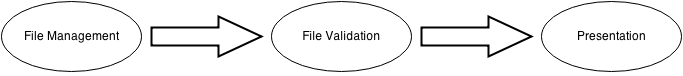
\includegraphics[scale=0.5]{evry-mickelson.png}
	\caption{Flow diagram}
	\label{fd}
\end{figure}

The problem is roughly divided in three phases as in \textit{Figure~\ref{fd}}. Each phase has a corresponding class described below - \textit{see Figure~\ref{cd}}. The provided source code is well documented, but this documentation should give a rough description of the implementation.

\begin{figure}
	\begin{center}
	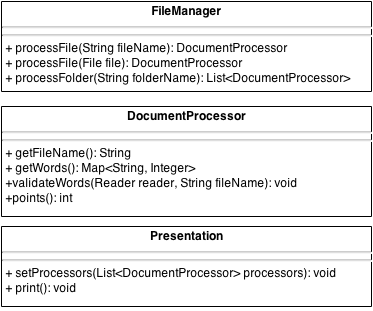
\includegraphics[scale=0.5]{cd.png}
	\caption{Class Diagram}
	\label{cd}
	\end{center}
\end{figure}

\subsection{Main class}
The Main class (defined as Main-Class in the MANIFEST file) mainly handles the input parameters and pushes the process forward in the flow as in \textit{Figure~\ref{fd}}. If the input parameters are for some reason wrong it will print usage information to the standard output.

\subsection{FileManager}
This class reads a file into a buffer and then passes it on to an instance of \textit{DocumentProcessor} (explained below). In the end it will return an instance of a \textit{DocumentProcessor} or a List of them, depending if it was invoked to read a file or a directory. In each case it only considers files with the extension {\bf.htm}, {\bf.html} or {\bf.txt}. On a single file it just needs to simply check the extension with simple \textit{String} manipulation. Reading a folder, the folder files are filtered using the interface \textit{FilenameFilter}. Then with a loop invoke the same functions as for a single file. 

For a HTML file the third party class Jsoup is used to strip HTML tags\cite{jsoup}.

\subsection{DocumentProcessor}
This class evaluates a single document, giving points as explained in the rules above and then storing this information for presentation in the last part of the flow in \textit{Figure~\ref{fd}}. The \verb:DocumentProcessor.validateWords: function takes a \textit{Reader} and filename and stores the filename and evaluates the words in the \textit{Reader}. All valid words are grouped by word and given points in a \textit{Map<String, Integer>}. The total points are stored in an encapsulated Integer.

Last thing worth noting on this class is that regular expressions were used to understand if a word contained a \textit{hyphen} or a \textit{double letter}. For this the standard \textit{Pattern} class together with the \textit{Matcher} class where used. The regular expression for a \textit{hyphen} is straight forward a \textit{"-"} character, the regular expression for \textit{double letter} is the more complex expression \textit{([a-zA-Z])\\1}.

\subsection{Presentation}
This class handles a list of \textit{DocumentProcessor} instances and presents to the standard output as in example in the \textit{Programmeringsuppgift} document. The class expones two functions, one to set the list of \textit{DocumentProcessor} instances and one \textit{print()} that simply prints to standard output. First the files with corresponding points in order of value and then the most \textit{important} words.

The sorting of words and documents are done in corresponding functions with an implementation of the interface \textit{java.util.Comparator}.

\newpage

\begin{thebibliography}{99}
	\bibitem{pdf}Anders Dannqvist\emph{Programmeringsuppgift} EVRY Consulting AB, 2014
	\bibitem{jsoup}jsoup\emph{Java HTML Parser} http://http://jsoup.org/
\end{thebibliography}

\end{document}
